\section{Process en bewaking}
Tijdens de afstudeerperiode is er gewerkt met een Agile \parencite{Agile} methode genaamd Scrum \Parencite{Scrum}.
Er is gewerkt met sprints van 2 weken waar bij de requirements opgedeeld werden in kleine stukjes.
Dit is gedaan om de taken behapbaar te maken en om snel veranderingen te kunnen aanbrengen.
Elke week werd er met de afstudeerbegeleider de progressie gesproken van de week waar bij mogelijk bijgestuurd werd.
De verschillende sprints werden bij gehouden in een notitie programma \textbf{Obsidian} hierbij is elke sprint opgedeeld in een apparte note.
Vervolgens is er gebruik gemaakt van een scrumboard om de progressie bij te houden dit werd ook gedaan in Obsidian.
In figuur \ref{fig:VoorbeeldSprint} is te zien hoe zo'n sprint ingepland werdt.

\whitespace[2]
\begin{graphic}
	\captionsetup{type=figure}
	\caption{Sprint 4 van het realisatie process}
	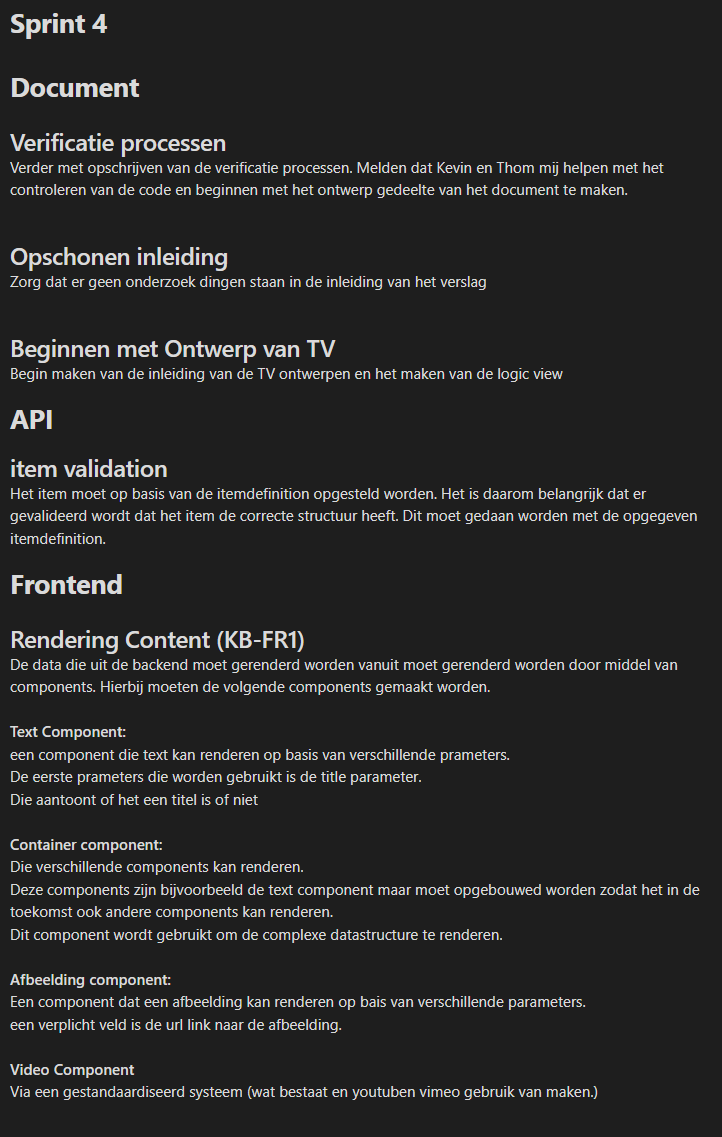
\includegraphics[scale=0.5]{SprintVoorbeeld.png}
	\label{fig:VoorbeeldSprint}
\end{graphic}

